% Plot of the hyperbolic tangent. tanh(x) goes to +/- 1 for x to +\- infinity while it is approximately linear for abs(x) < 1.
% Appears in many places in physics, e.g. in the magnetization of an ideal paramagnet of independent spins.

\documentclass{standalone}

\usepackage{pgfplots}
\pgfplotsset{compat=newest}

\begin{document}
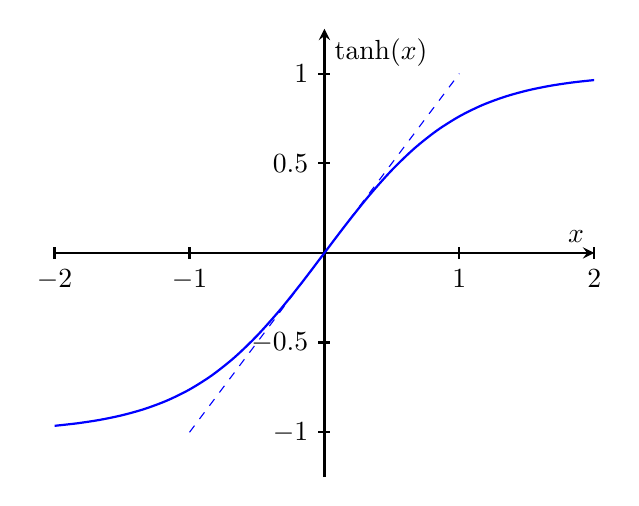
\begin{tikzpicture}
  \begin{axis}[
      xlabel = $x$,
      ylabel = $\tanh(x)$,
      ymin = -1.25,ymax = 1.25,
      domain = -2:2,
      smooth,thick,
      axis lines = center,
      every tick/.style = {thick}]

    \addplot[color=blue]{tanh(x)};
    \addplot[color=blue,dashed,domain=-1:1,thin]{x};

  \end{axis}
\end{tikzpicture}
\end{document}